\subsection{Spielmodis}

Die loolou Erweiterung hat vier verschiedene Modi zum Spielen. Diese k"onnen w"ahrend dem Spiel einfach "uber den Drucktaster am Oberteil der Spielbasis umgeschaltet werden.
Die vier roten LEDs neben dem Drucktaster zeigen dabei den aktuellen Modus an. \\
Die folgende Tabelle beschreibt die 4 verschiedenen Modi.

\vspace{1cm}
\begin{table}[ht]
	\centering

	\begin{tabular}{ c | p{8cm} } 
		% table header
		Modus								& Beschreibung \\ 
		\hline \hline
		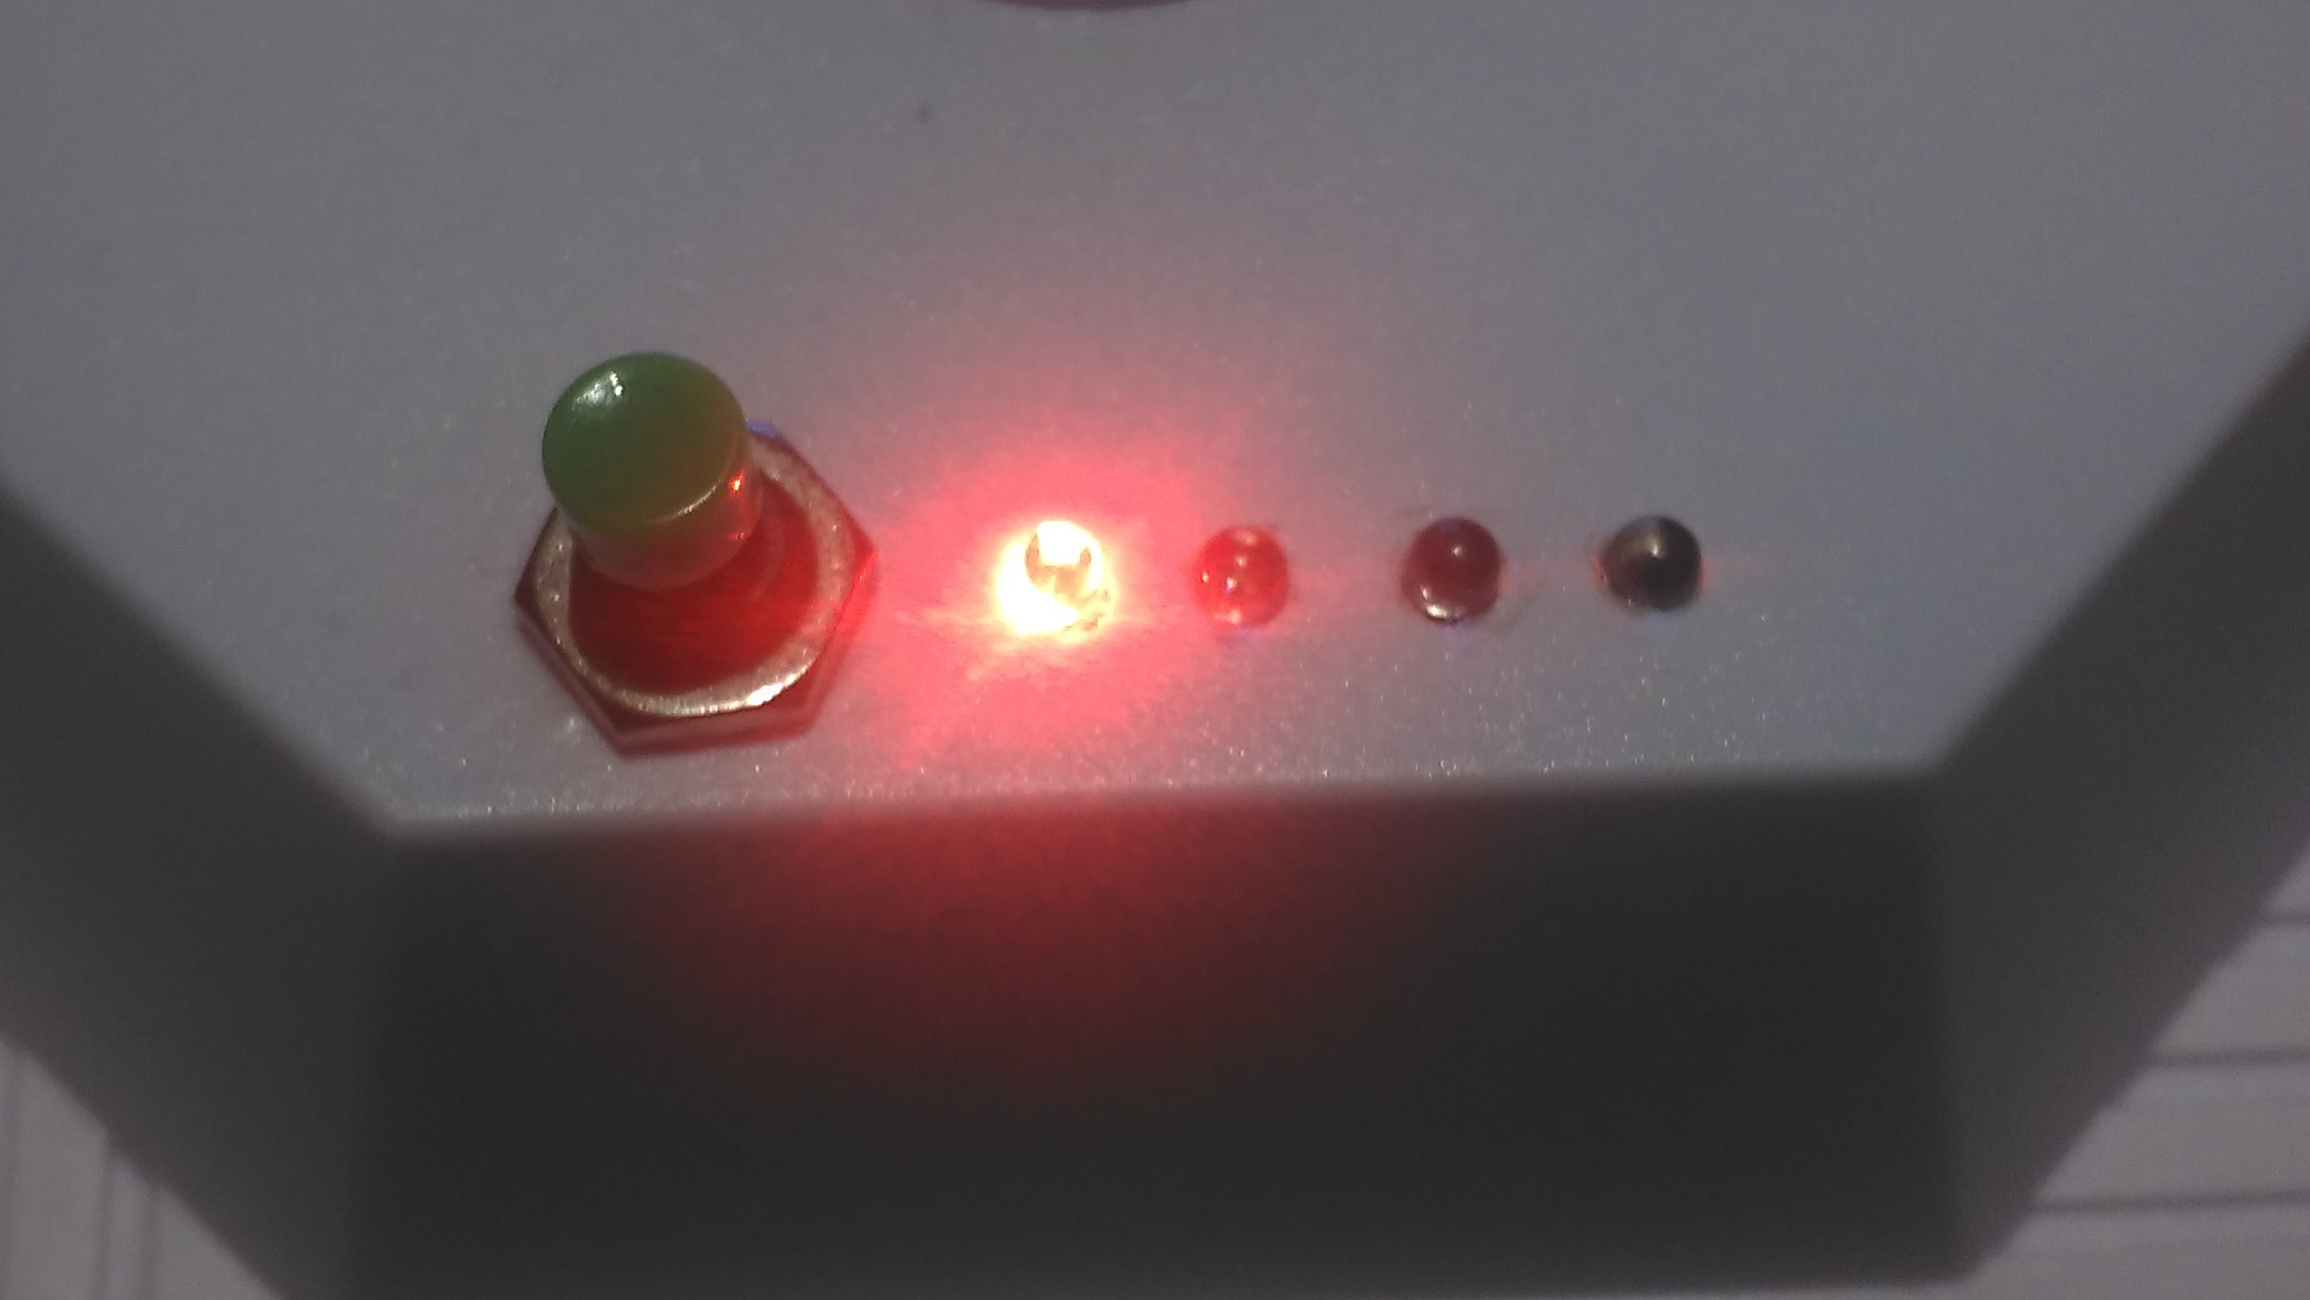
\includegraphics[width=0.2\textwidth]{pictures/mode_1.jpg}	& Einfacher Modus.\newline Looping Louie dreht sich so schnell wie beim originalen Spiel.  \\
		\hline
		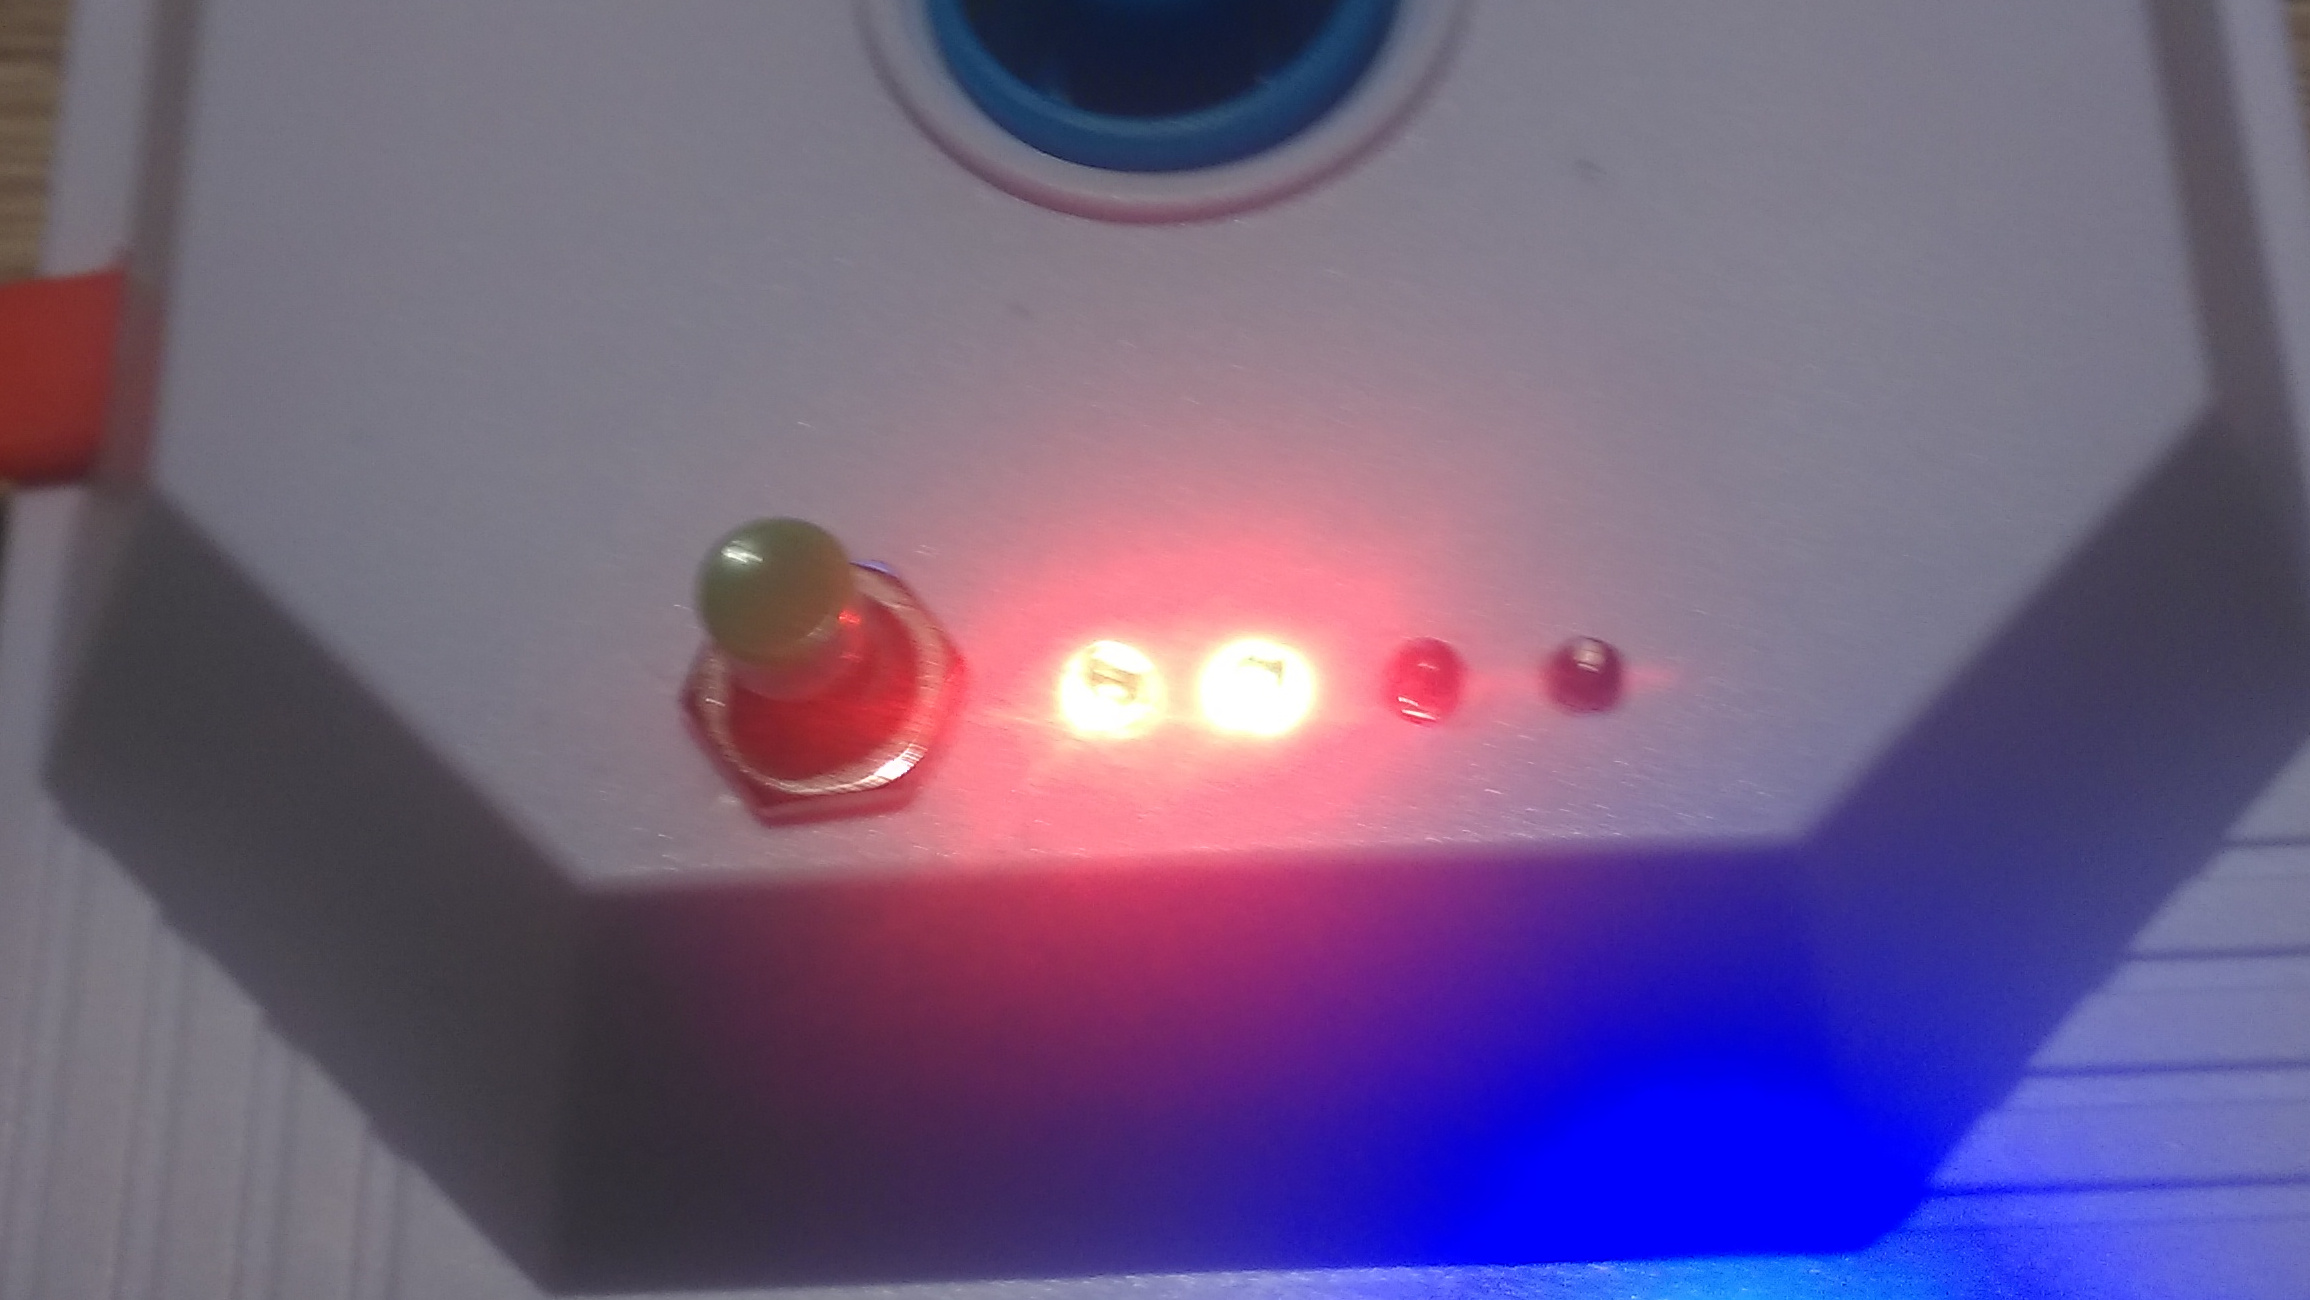
\includegraphics[width=0.2\textwidth]{pictures/mode_2.jpg}	& Schneller Modus.\newline Looping Louie dreht sich viel schneller als gewohnt. \\
		\hline
		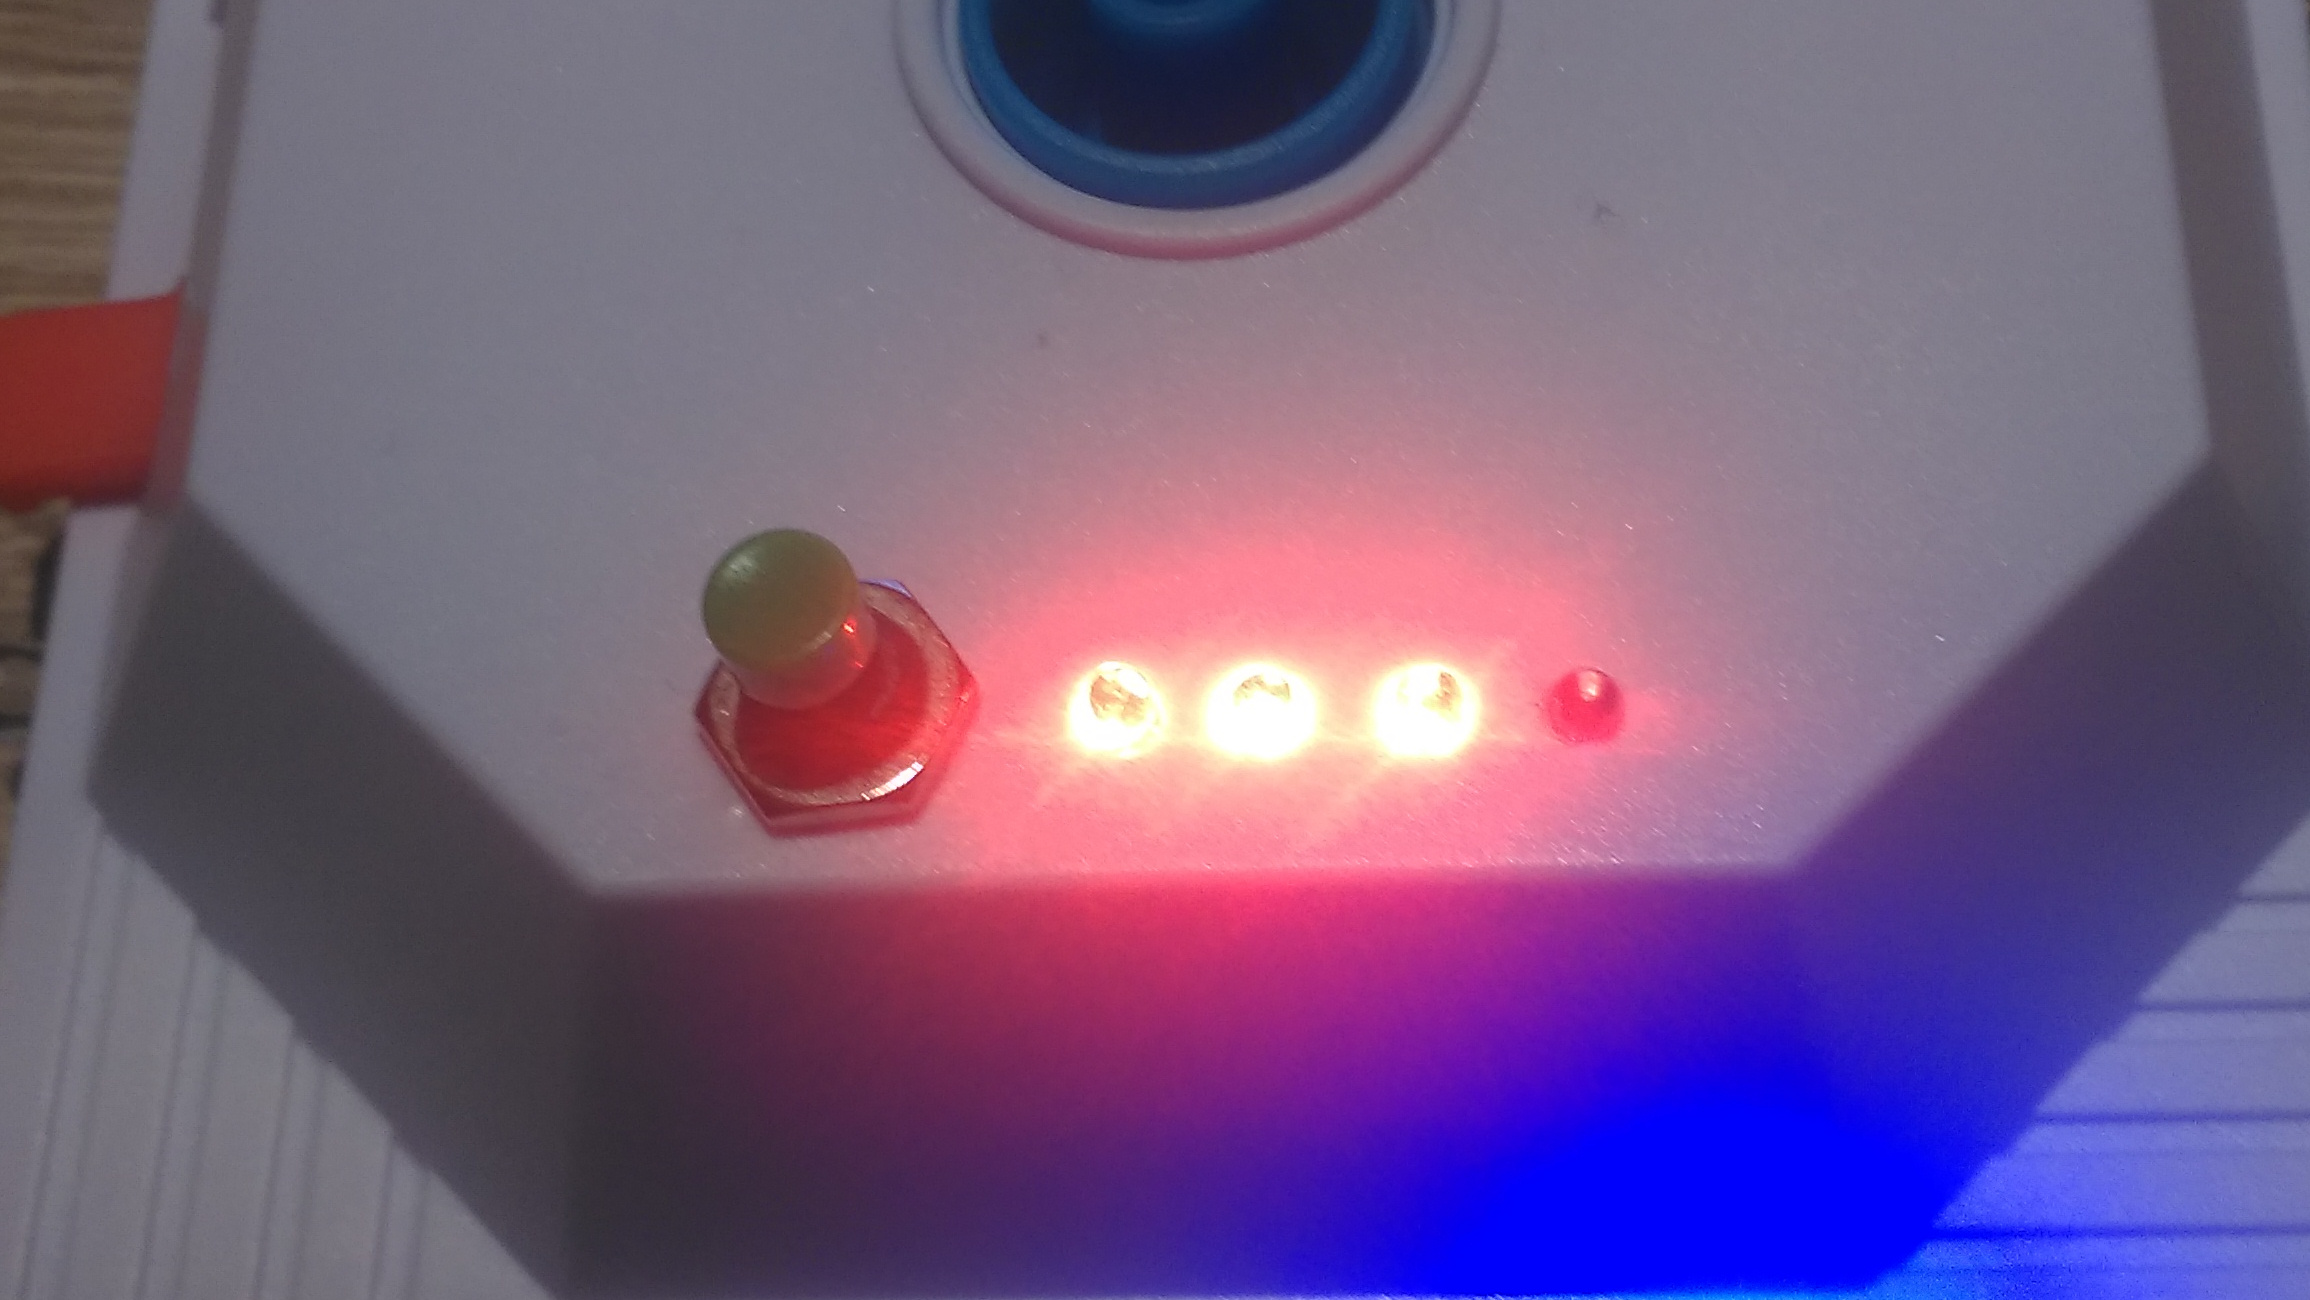
\includegraphics[width=0.2\textwidth]{pictures/mode_3.jpg}	& Zuf"alliger Modus.\newline Looping Louie "andert seine Gewschwindigkeit und bleibt auch mal stehen. \\
		\hline
		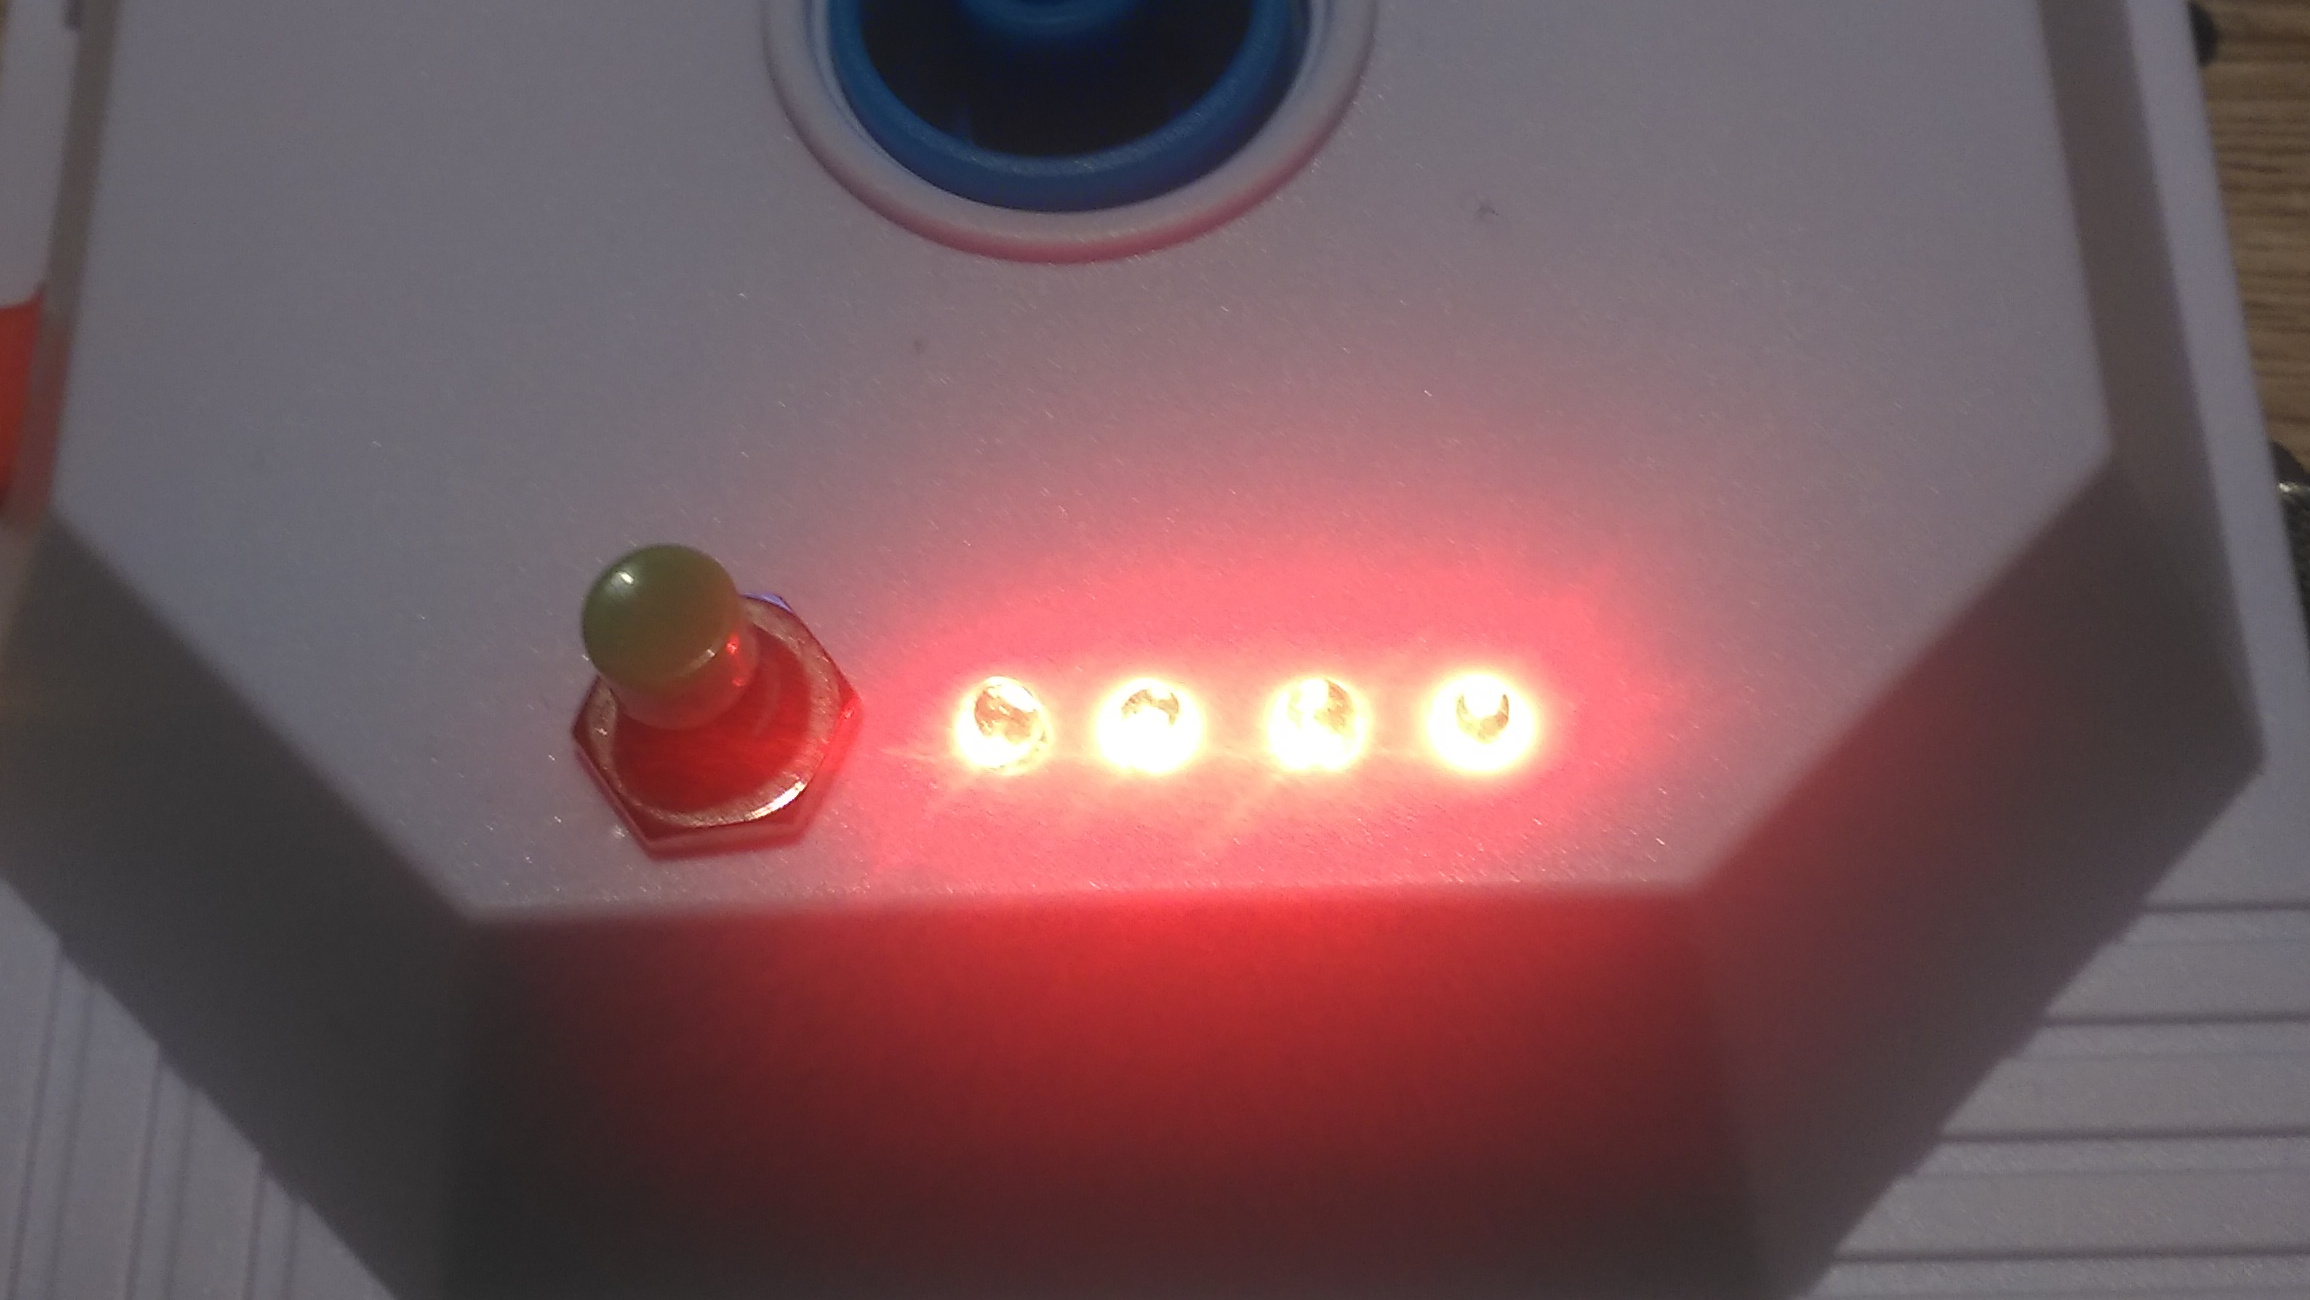
\includegraphics[width=0.2\textwidth]{pictures/mode_4.jpg}	& Zuf"alliger Modus mit R"uckw"artsgang.\newline Looping Louie "andert seine Geschwindigkeit und Richtung. \\
		\hline
	\end{tabular}

	\caption{Spielmodi}
	\label{table:mode}
\end{table}
\vspace{0.5cm}

\newpage
\subsection{Source code}

Der Source-Code von loolou ist ver"offentlich und kann heruntergeladen und selbst kompiliert werden.
Bitte beachten Sie die Lizenz von loolou. Zu finden ist diese im Kapitel ~\ref{section:licence} auf Seite ~\pageref{section:licence}.
\subsubsection{Github}\label{subsubsection:github}

Der Source-Code ist auf Github ver"offentlich und kann unter folgendem Link heruntergeladen werden. \\
\begin{center}\href{https://github.com/berauser/loololu}{https://github.com/berauser/loololu}\end{center}
\vspace{0.5cm}

\subsubsection{Defines}

Die defines sind in der Datei main.c definiert. Sie definieren die PINs und PORTs der LEDs, PWMs und des Drucktasters f"ur den ATTINY2313.
Ebenso werden hier die Timer-Delays und PWM-Frequenzen f"ur den Spielablauf definiert. Das folgende Listing (Listing ~\ref{lst:defines}) zeigt alle, f"ur den Spielablauf wichtigen, Defines. 

\vspace{0.5cm}
\begin{lstlisting}[caption={Defines},label=lst:defines]
// ********************************************************
// PWM values
// ********************************************************
#define PWM_OFF   0 // 0V ( OFF )
#define PWM_3V   85 // 3V ( (9V / 255) * 85 = 3V )
#define PWM_9V  255 // 9V


// ********************************************************
// PWM values
// ********************************************************
//
//   1000000Hz ( F_CPU )
//  --------------------- = 976,56 ( 0x3D0 )
//   1024 * 1Hz (1 sec)
#define TIMER_INT_DEPLAY 0x3D0

// ********************************************************
// Pin description
// ********************************************************
//
//		  attiny 2313
//           ---------------------
//  RESET   -| 1 (PA2)  (VCC) 20 |- VCC
//  LED5    -| 2 (PD0)  (PB7) 19 |- SCK
//  LED6    -| 3 (PD1)  (PB6) 18 |- MISO
//  LED7    -| 4 (PA1)  (PB5) 17 |- MOSI
//  LED8    -| 5 (PA0)  (PB4) 16 |- FORWARD
//  BUTTON  -| 6 (PD2)  (PB3) 15 |- BACKWARD
//  NC      -| 7 (PD3)  (PB2) 14 |- PWM
//  LED1    -| 8 (PD4)  (PB1) 13 |- LED4
//  LED2    -| 9 (PD5)  (PB0) 12 |- LED3
//  GND     -| 10(GND)  (PD6) 11 |- NC
//           --------------------
//

// *** LEDs ***********************************************
#define PIN_LED1 PD4
#define PIN_LED2 PD5
#define PIN_LED3 PB0
#define PIN_LED4 PB1
#define PIN_LED5 PD0
#define PIN_LED6 PD1
#define PIN_LED7 PA1
#define PIN_LED8 PA0

#define PORT_LED1 PORTD
#define PORT_LED2 PORTD
#define PORT_LED3 PORTB
#define PORT_LED4 PORTB
#define PORT_LED5 PORTD
#define PORT_LED6 PORTD
#define PORT_LED7 PORTA
#define PORT_LED8 PORTA

#define DDR_LED1 DDRD
#define DDR_LED2 DDRD
#define DDR_LED3 DDRB
#define DDR_LED4 DDRB
#define DDR_LED5 DDRD
#define DDR_LED6 DDRD
#define DDR_LED7 DDRA
#define DDR_LED8 DDRA

// *** DIRECTION / PWM ************************************
#define PIN_DIRECTION_FORWARD  PB4
#define PIN_DIRECTION_BACKWARD PB3
#define PIN_PWM                PB2

#define PORT_DIRECTION_FORWARD  PORTB
#define PORT_DIRECTION_BACKWARD PORTB
//#define PORT_PWM

#define DDR_DIRECTION_FORWARD  DDRB
#define DDR_DIRECTION_BACKWARD DDRB
#define DDR_PWM                DDRB

#define REGISTER_PWM  OCR0A
#define MODE_PWM      (1 << COM0A1) | (1 << WGM00)
#define CLOCK_PWM     (1 << CS01)

#define REGISTER_TIMER OCR1A
#define MODE_TIMERA    0x00
#define MODE_TIMERB    (1 << WGM12) | (1 << CS12) | (1 << CS10) // clk/1024

// *** BUTTON *********************************************
#define PIN_BUTTON  PD2
#define PORT_BUTTON PORTD
#define DDR_BUTTON  DDRD
#define EDGE_TYPE_BUTTON (1 << ISC01) // interrupt on falling egde
\end{lstlisting}
\vspace{0.5cm}

\subsubsection{Main-Methode}

Im Listing ~\ref{lst:main} ist die main-Funktion des Programmes. Diese initialisiert die Peripherie und springt dann in eine while-true-loop.
Die while-true-loop setzt in jeden Durchlauf die aktuelle Geschwindigkeit und schaltet die LEDs f"ur die Richtungsanzeige ein, beziehungsweise aus. Anschlie"send werden 250ms gewartet bis die n"achste LED f"ur die Richtungsanzeige eingeschaltet wird. 

\vspace{0.5cm}
\begin{lstlisting}[caption={Main-Method},label=lst:main]
// ****************************************************************************
// game
// ***************************************************************************/
int main(void) {

	init();
	setup();

	/* main loop */
	while (1) {
		/* all other uses interrupts */
		trigger_speed( speed );
		trigger_direction( direction );
		show_direction( direction );
		_delay_ms( 250 );
	}

	return 0;
}
\end{lstlisting}
\vspace{0.5cm}

\subsubsection{Init-Methode}

Die Methode init initialisert die GPIOs (General Porpuse Input/Output) des ATTINY.

\vspace{0.5cm}
\begin{lstlisting}[caption={Setup-Method},label=lst:setup]
// ****************************************************************************
// initialize gpio, set pin directions
// ***************************************************************************/
void init( void )
{
	// leds
	GPIO_init( DDR_LED5, PIN_LED5, OUTPUT ); // 1
	GPIO_init( DDR_LED6, PIN_LED6, OUTPUT ); // 2
	GPIO_init( DDR_LED7, PIN_LED7, OUTPUT ); // 3
	GPIO_init( DDR_LED8, PIN_LED8, OUTPUT ); // 4

	GPIO_init( DDR_LED1, PIN_LED1, OUTPUT ); // red
	GPIO_init( DDR_LED2, PIN_LED2, OUTPUT ); // blue
	GPIO_init( DDR_LED3, PIN_LED3, OUTPUT ); // green
	GPIO_init( DDR_LED4, PIN_LED4, OUTPUT ); // yellow

	// motor control
	GPIO_init( DDR_DIRECTION_BACKWARD, PIN_DIRECTION_BACKWARD, OUTPUT ); // backward
	GPIO_init( DDR_DIRECTION_FORWARD,  PIN_DIRECTION_FORWARD,  OUTPUT ); // forward
	GPIO_init( DDR_PWM, PIN_PWM, OUTPUT ); // PWM
	PWM_enable( MODE_PWM, CLOCK_PWM, REGISTER_PWM, PWM_OFF );

	// button
	GPIO_init( DDR_BUTTON, PIN_BUTTON, INPUT);
	GPIO_interrupt( PORT_BUTTON, PIN_BUTTON, INT0, EDGE_TYPE_BUTTON );

	// timer interrupt
	TIMER_enable( MODE_TIMERA, MODE_TIMERB );

	// Enable interrupts
	sei();
}
\end{lstlisting}
\vspace{0.5cm}

\subsubsection{Setup-Methode}

Die Setup-Methode initialisert das loolou-Programm mit den default-Werten.

\vspace{0.5cm}
\begin{lstlisting}[caption={Init-Method},label=lst:init]
// ****************************************************************************
// setup syStem with default values
// ***************************************************************************/
void init( void )
{
	// set initial values
	active_led  = LED1;
	mode        = M_NORMAL_FORWARD;
	speed       = PWM_3V;
	direction   = FORWARD;

	// show current mode
	show_mode();

	// set seed
	init_random( TCNT1L );

	// initial pwm
	trigger_speed( PWM_3V );

	// set initial timer delay
	TIMER_set( TIMER_INT_DEPLAY );
}
\end{lstlisting}
\vspace{0.5cm}

\subsubsection{Interrupt Service Routine}

Das Programm loolou implementiert zwei verschiedene Interrupt Service Routinen (ISR) - die ISR(INT0\_vect) und ISR(TIMER1\_COMPA\_vect). \\
Die ISR(INT0\_vect) wird bei einer fallenden Flanke am Drucktaster aufgerufen. In der ISR(INT0\_vect) wird der Modus des Spieles um eins hochgez"ahlt und neu ausgegeben. Anschlie"send wird der Timer zur"uckgesetzt und aufgerufen um die neue Geschwindigkeit und Spiel-Richtung zu setzen. \\
Die Interrupt Service Routine ISR(TIMER1\_COMPA\_vect) wird jede Sekunde aufgerufen und berechnet die Geschwindigkeit und die Spiel-Richtung neu.

\vspace{0.5cm}
\begin{lstlisting}[caption={Interrupt Service Routine},label=lst:isr]
// ****************************************************************************
// interrupt service routine
// ***************************************************************************/
ISR(INT0_vect)
{
	ADD_ONE_BETWEEN( mode, M_NORMAL_FORWARD, M_RANDOM_RANDOM );
	show_mode();

	/* reset timer, call ISR to change speed/direction immediately */
	TIMER_reset();
	TIMER1_COMPA_vect();
}

ISR(TIMER1_COMPA_vect)
{
	direction = calc_direction();
	speed = calc_speed();
}
\end{lstlisting}
\vspace{0.5cm}

\subsubsection{Calculate direction Methode}

Die Funktion calc\_direction gibt anhand des aktuellen Spielmodus die Spiel-Richtung zur"uck.
F"ur die drei Spielmodis \grqq{}Einfacher Modus\grqq{}, \grqq{}Schneller Modus\grqq{} und \grqq{}Zuf"alliger Modus\grqq{} wird immer die Spiel-Richtung \grqq{}forw"arts\grqq{} ausgeben.
Im Spielmodus \grqq{}Zuf"alliger Modus mit R"uckw"artsgang\grqq{} wird anhand einer Zufallszahl die Spiel-Richtung berechnet. In diesem Modus wird etwa 10\% \grqq{}r"uckw"arts\grqq{} und etwa 90\% \grqq{}forw"arts\grqq{} zur"uckgegeben.

\vspace{0.5cm}
\begin{lstlisting}[caption={Calculate direction},label=lst:calcdirection]
// ****************************************************************************
// calculates a new direction
// ***************************************************************************/
GameDirection calc_direction( void )
{
	switch( mode )
	{
		case M_NORMAL_FORWARD:
		case M_FAST_FORWARD:
		case M_RANDOM_FORWARD:
		default:
			return FORWARD;
			break;
		case M_RANDOM_RANDOM:
			return ( (get_random_between( 0, 10 ) == 0) ? BACKWARD : FORWARD ); /* 10% backward : 90% forward */
			break;
	}
}
\end{lstlisting}
\vspace{0.5cm}

\subsubsection{Calculate speed Methode}

Die Funktion calculate\_speed gitb anhand des Spielmodus die berechnete Geschwindigkeit zur"uck.
Im Modus \grqq{}Einfacher Modus\grqq{} wird immer der PWM-Wert f"ur 3V und im Modus \grqq{}Schneller Modus\grqq{} der PWM-Wert f"ur 9V zur"uckgeliefert.
In den Spielmodis \grqq{}Zuf"alliger Modus\grqq{} und \grqq{}Zuf"alliger Modus mit R"uckw"artsgang\grqq{} wird die Geschwindigkeit anhand zweier Zufallszahlen berechnet.
Dabei wird die erste Zufallszahl f"ur die grobe Einordnung der Geschwindigkeit verwendet und die zweite Zufallszahl f"ur die exakten PWM-Wert, der dann auch zur"uckgegeben wird. Die erste Zufallszahl ist in dieser BErechnung notwendig um gr"o"sere Spr"unge zwischen den Geschwindigkeiten zu reduzieren. 
Die Werte sind wie folgt aufgeteilt: Etwa 10\% zwischen 0.0V und \~{}3.5V, etwa 70\% zwischen \~{}3.5V und \~{}7.0V, sowie 20\% zwischen \~{}7.0V und \~{}9.0V. 

\vspace{0.5cm}
\begin{lstlisting}[caption={Calculate Speed},label=lst:calcspeed]
// ****************************************************************************
// calculates a new speed
// ***************************************************************************/
uint8_t calc_speed( void )
{
	switch( mode )
	{
	case M_NORMAL_FORWARD:
	default:
		return PWM_3V;
		break;
	case M_FAST_FORWARD:
		return PWM_9V;
		break;
	case M_RANDOM_FORWARD:
	case M_RANDOM_RANDOM:
	{
		/*
		 * Calculate speed in 25 steps.
		 * 0 = 0V, ...,  25 = ~9V
		 *
		 * For a better and faster playing pleasure,
		 * a probability of
		 * 10% values between   0V and 3,5V and
		 * 70% values between 3,5V and 6,0V is selected.
		 * 20% values between 7,0V and 9,0V is selected.
		 */
		static uint8_t r = 0;
		r = get_random_between( 0, 10 );
		if ( r == 0 )
		{ /* 20% slow ( 0V - ~3,5V ) */
			return get_random_between(  0, 100 );
		}
		else if ( r == 1 || r == 2 )
		{ /* 20% very fast /~7,0V - 9,0V */
			return get_random_between( 201, 255);
		}
		else
		{ /* 70% fast ( ~3,5V - ~7,0V ) */
			return get_random_between( 101, 200 );
		}
	}
		break;

	}
}
\end{lstlisting}
\vspace{0.5cm}

\subsection{Kompilieren des Sourcecodes}
\subsubsection{Abh"angigkeiten an das Buildsystem}

Um den C-Sourcecode f"ur den ATTINY2313 zu "ubersetzen werden einige wenige Anfoderungen an das Buildsystem gestellt.
Es wir lediglich die AVR-Toolchain (avr-gcc) und ein Programmer f"ur Atmel-Mikrocontroller ben"otigt (avrdude).
Um die Dokumentation zu erstellen wird zus"atzlich ein LaTeX-Kompiler ben"otigt, unter Ubuntu oder Debian bietet sich hier zum Beispiel texlive an.\\
\\
F"ur Ubuntu und Debian k"onnen die folgenden Befehle, zum installieren der Abh"angigkeiten, verwendet werden.

\vspace{0.5cm}
\begin{lstlisting}[caption={Build dependencies},language=sh,label=lst:builddep]
# install avr toolchain and avr programmer
sudo apt-get install gcc-avr avrdude
# install LaTeX-Compiler
sudo apt-get install texlive-full
\end{lstlisting}
\vspace{0.5cm}

\subsubsection{Kompilieren}

Das Kompilieren des C-Sourcecodes durch einen einfachen Make-Aufruf angesto"sen werden.
Dazu muss im Root-Verzeichniss des Sourcecodes folgender Befehl eingegeben werden.

\vspace{0.5cm}
\begin{lstlisting}[caption={Compile},language=sh,label=lst:makeall]
# compile loolou
make
\end{lstlisting}
\vspace{0.5cm}

\subsubsection{Aufr"aumen}

Um die Kompilierten Source wieder zu l"oschen kann der folgende Befehl verwendet werden.

\vspace{0.5cm}
\begin{lstlisting}[caption={Clean},language=sh,label=lst:makeclean]
# clean loolou sources
make clean
\end{lstlisting}
\vspace{0.5cm}

\subsubsection{Erstellen der Dokumentation}

Das erstellen der Dokumentation kann ebenso wie das kompilieren des Sourcecodes durch einen Make-Aufruf ausgef"uhrt werden.
Dazu f"ugt man das Schl"usselwort \grqq{}doc\grqq{} dem \grqq{}make\grqq{} an.

\vspace{0.5cm}
\begin{lstlisting}[caption={Create documentation},language=sh,label=lst:builddoc]
# create documenation
make doc
# clean documenation
make doc-clean
\end{lstlisting}
\vspace{0.5cm}


\subsection{Wie der Attiny2313 programmiert wird}
\subsubsection{Programming}

Ebenso wie das Kompilieren der Source kann der Attiny mittels eines vordefinierten Make-Aufrufs programmiert werden.
Dies kann "uber den Befehl \grqq{}make burn\grqq{} ausgef"uhrt werden.
Mittels den Variablen \textbf{AVRDUDE\_PROGRAMMER} und \textbf{AVRDUDE\_PORT} kann das Device und der Programmer-Typ definiert werden.
Die Default-Einstellungen sind \textbf{avrispv2} f"ur den Typ des Programmers und \textbf{/dev/ttyAMC0} f"ur das Device.
Der Typ des Programmers kann der Dokumentation des Programmers entnommen werden. \\
\\
\textbf{Achtung: Sollte der Programmer eine eigene Stromversorgung f"ur den Attiny haben, dann darf der 9V Stromanschluss des Looping Louie nicht angeschlossen werden}, wenn das Programmieren "uber die eingebaute Programmier-Schnittstelle (J1) stattfindet. Andernfalls kann der Programmer besch"adigt werden.

\vspace{0.5cm}
\begin{lstlisting}[caption={Programming},language=sh,label=lst:makeburn]
# flash the attiny (using default values)
make burn
# or
make AVRDUDE_PROGRAMMER=avrispv2 AVRDUDE_PORT=/dev/ttyAMC0 burn
# AVRDUDE_PROGRAMMER define programmer type
# AVRDUDE_PORT define programmer device
\end{lstlisting}
\vspace{0.5cm}



